%\chapter{The world of Code}
\chapter{How to write code}
\label{chap:worldcode}

\begin{abstract}{Abstract}
  
Programming is no longer a solitary activity, and almost all questions, problems, and error messages have been encountered and solved before. This chapter explains the most common forms of collaboration and sources of outside help, as well as giving best practices on how to write and share code yourself.
\end{abstract}

\keywords{package, library, errors, computational hygiene, notebooks}

\begin{objectives}
\item Understand the importance of re-using code when programming
\item Help first coders to avoid getting stuck
\item Explain "computational hygiene" and show best practices in R and Python to write and share code
\end{objectives}

In the \refchap{programmingconcepts}, you have learned how to write
your first lines of code.  You created objects of different types,
used and wrote some functions, and explored the major control structures.
You are probably eager to write your first longer piece of code and
produce some interesting data processing or analysis script. In this
chapter, we prepare you to do this with as little frustration as possible.
You will be introduced to some best practices so that you can implement
them right from the start and to some tools that make your life easier.

First, we will answer the question how you avoid reinventing
the wheel: When is it appropriate to simply use someone else's existing code, and
when do you need to write your own code from scratch? And is there a middle ground?

Second, we will discuss how to turn error messages -- which you will inevitably
see a lot -- from a frustrating annoyance into a helpful tool.

Finally, we will discuss some best practices when writing code.

\section{Re-using code: How not to re-invent the wheel}
\label{sec:code}

Just as any human language, also programming languages consist of a vocabulary, syntax rules, and expressions. Using the proper words and grammar, you can build from scratch any idea your imagination allows you. That's a wonderful thing! But, let's be honest: The language itself, the expressions, ideas, and all the abstract constructs seldom come originally from you. In fact, that's great as well: Otherwise, you'd have to deeply think of every element before talking and expressing any thought. Instead, you use pre-existing rules, ideas, perceptions and many different narratives to create your own messages to interact with the world. It's the same with coding: You never start from scratch.

Of course you \emph{can} code anything you want from the very beginning, even just using 0's and 1's!
When reading through the previous chapters, maybe you even started to think that complex operations will be very exhausting and will take a really long time. After all, from the basic operations we did to a useful statistical model seems like a long way to go.

Luckily, this is not the case.
There is almost no project in which computational scientists, data analysts, or developers do not re-use earlier code in order to achieve their goals quicker and more efficiently.
The more common a task is, the greater the chance that you do not have to re-invent the wheel.
Of course, you have to give credit where credit is due, but it is not uncommon to paste code snippets from others into your own code and adapt them. This is especially true for standard operations, for which there are only so-many ways to do achieve the desired result.

There are different ways to re-use earlier code. One is to copy and adapt raw lines of code written by someone else or by yourself in the past. In fact, there are many online repositories such as Github or BitBucket that contain many programs and well-documented code examples (see \refsec{practices}). When conducting computational analyses, you will spend a significant part of your time in such repositories trying to understand what others have done and figuring out how you can use it in your own work. Of course, make sure that the license of the code allows you to use it in the way you want. Also, give credit where credit is due: At the very least, plase a comment with a link in your code to indicate what inspired you.

Another way is to build or import functions that summarize many lines of code into a simpler command, as we explained in \refsec{functions}. The functions are indeed powerful strategies to re-use the code since you do not have to write the same code over and over again if you need it in multiple places. Packages are probably the most elegant approach to recycle the work made by other colleagues. In \refsec{installing} you already learnt how to install a package and you did probably noticed how easy it is to bring many pre-build functionalities onto your workspace. You can also write and publish your own package in the future to help your colleagues to write less code and to be more efficient in their daily job (see also \refsec{publishingsource})!

A lot of questions can arise here: What to re-use? When to use a function written by someone else instead of writing the code yourself? Which scripts and sources are trustworthy? Which is the best package to choose? How many packages should we use within the same project? Should we care about package versions? And must we know every package that is released in our field? There are of course multiple answers to these questions and it will be probably a matter of practice how to obtain the most appropriate ones. In general, we can say that one premise is to re-use and share code as much as you can. This idea is limited by constraints of quality, availability, parsimony, updates and expertise. In other words, when recycling code we should think of the reputation of the source, the difficulty to access it, the risk of having an excessive and messy number of inputs, the need to share the last developments with your colleagues and the fact that you will never be able to know everything.

Let's take an example. Imagine you want to compute the Levenshtein distance between two
strings. That's a pretty straightforward metric that answers the question: ``How many
edits (removing/changing/editing characters) do I need to apply to transform string1 into string2?''
It can be used for plagiarism detection, but may be interesting for us to determine, for instance,
whether a newspaper copied some content from somewhere else, even if small changes have been
applied. You could now try to write some code to calculate that (and we are sure you could
do that if you invested some time in it!), but it is such a common problem that it
has been solved multiple times before. You could, for instance,  look up some
functions that are known to solve the problem and copy-paste them into your code. You can find
a large number of different implementations for both Python and R here:
\url{https://en.wikibooks.org/wiki/Algorithm_Implementation/Strings/Levenshtein\_distance}.
You can then choose and copy-paste the one which is most appropriate for you. One that is very fast, because
you want to compare a huge set of strings? One that is easy to understand? One that uses
only a few lines of code to not distract the reader?
Alternatively, if you look for available packages for Python and R, you see that there are
multiple packages that you can install with \fn{install.packages} (R) or \fn{pip} (Python)
and then import. If you go for that route, you don't need
to care about the internal workings and can ``abstract away'' and outsource the problem -- on the other
hand, the users of your code now have one more dependency to install before they can
use your code.

In the case of package selection, we understand it can be quite overwhelming,
with so many different packages from different contributors.
In fact, sometimes the same task, such as topic modeling,
can be done using multiple different packages.
So, how to find and choose the best package?
Besides resources like this book, the most important guide is probably the community around you:
using packages that a lot of other people also use means that the package is probably well maintained and documented,
and that there is a community to ask for help if needed.
Since all packages on Pypi and CRAN are free to download and install, however, you can also shop around and see what the various packages do.
When comparing different packages, it is always good to check their documentation and their github page:
packages that are well documented and that are updated frequently are often a good choice.

Just to mention an example, the authors of this book had several intensive discussions of which packages to mention and use in the proposed exercises, an issue that became complex given the variety of topics addressed in this book. In the case of text analysis, a library such as \fn{NLTK} for Python was incredibly popular among computational analysts until a few years ago becoming a package of reference in the field, but it has -- at least for some applications -- been overpassed by friendly and sophisticated new packages for natural language processing like \fn{SpaCy}. So, which should we have included in this book? The one which is well-known (with excellent documentation by the way) and still used by thousands of practitioners and students around the world, or the one which is penetrating the market because of its easiness and advantages? Moreover, when choosing the second option, are we sure a more trendy package is going to be stable in time or is it going to be crossed out by a different one in just few months?  

There isn't the one golden way of how to re-use code and packages, but this dynamic scenario also depicts an exciting and provocative field that forces us to keep ourselves updated.


\section{Understanding errors and getting help}
\label{sec:errors}


Programming can be a frustrating endeavour, and you will encounter error messages, bugs, and problems that you don’t know how to fix. This section shows how error messages are useful rather than scary and lists the main error messages encountered in the beginning. It explains how to search for help within the R/Python documentation, how to use online resources, and how to formulate questions to your instructor or community so you get a useful answer. 

\section{Best practices: beautiful code, GitHub, and notebooks}
\label{sec:practices}


This section gives a brief explanation of ``computational hygiene'': how to structure your code such that you can understand it later, the importance of naming and documentation, the use of versioning and online repositories such as GitHub, and the use of literate programming (Rmd/Jupyter notebooks) to explain, share and publish code.

Coding is more than learning the basic rules and creating a message. If you want use the code to communicate ideas and to work with peers you have to take care of many content and shape details in order to guaranty the comprehension and reproducibility of the scripts. It even applies to the code you write for "private use" because it is highly likely that you forget your original thoughts from one day to another, or that you later realize that you need to share it with someone else to ask for help. Thus instead of writing personal, hidden and \textit{illiterate} code without adopting any social conventions, you should dedicate some extra effort to have your scripts easy and ready to share.

The first step of the computational hygiene is within the very code. Every time you create an object, a variable or a function you have to take many apparently unimportant decisions when giving a name, separating words, lines or blocks, and including comments. These decisions are personal but mostly should depend on social conventions in order to be useful. As you may imagine, it exists many of these conventions for general programming and specially for specific languages. Just to mention some, you can find a "official" style guide for Python\footnote{https://www.python.org/dev/peps/pep-0008/}  or a Google's R style guide\footnote{https://google.github.io/styleguide/Rguide.html}. Some of these guides are extensive (they cover every detail) and some are more general or abstract, and they are not properly a "bible" or a rule of thumb for practitioners, but orientate  coders for best practices. In fact, even when you find them useful it is true that you will probably learn more of these practices from reading good examples and specially from interacting with a specific community and its rules.

We will mention some general guidelines that apply for both R and Python. If it is the first time you are into the world of code you will find these advices useful,  but if you are a more advanced learner you will probably get more specific knowledge in more detailed sources for each language and community.

In the case of naming we encourage you to use meaningful names or standard abbreviations to objects, using lower-case or mixed-case (remember it's case-sensitive!), avoiding special characters and operators (such as \&, @ or \%), and not exceeding 32 characters. You normally begin with a letter (an upper-case when defining a class or even with an underscore for private identifiers), followed by other letter or numbers, and using underscores to separate the words if it is necessary (i.e. \texttt{data\_2020} or \texttt{Filter\_Text}). Some suggest that variable names should be nouns and function names should be verbs, which seems logical if you think of the nature of these objects. 

When writing the code, please take also into consideration the white spaces and indentations (remember 2 spaces for R and 4 for Python!), because you should use them to give proper structure to the code by creating the block statements (in the case of R also pay attention to the use of curly braces\footnote{The convention is that the opening curly begins after some code and is always followed by a new line; and the closing curly is in its own line except if there are more instructions in the block}). Do not write very long lines (more than 80 characters) to help your code fit the screen and avoid lateral scrolling. Good separation of words, lines and blocks will make your script more readable!

Now, if you want to make your code highly understandable and shareable, you have to include \textit{documentation}.
This is probably a very basic dimension of coding but unfortunately some authors forget to include some few words of what they have done in their scripts, making your journey (and sometimes their own!) more difficult.
An essential good practice in coding is to include enough information that clarify your code when it is not clear by itself.
You can do this in different ways (even by writing a separate codebook), but the most natural and straightforward manner is to include some  \textit{comments} in the code.
This comments should be included both at the beginning of the script to give an overview or introduction to the code;
and within the script (in independent lines or at the the end of a line) to give specific orientations.
A

R and Python use the hash sign \texttt{\#} to create these comments. Notice that the comment will begin always after the hash, so this part will not be executed when compiling. If the first character in your line is  a \texttt{\#} all the text included will be considered as a comment; but if you have already written some code in a line and include a \texttt{\#} after the code, the initial code will be executed and you will always see the comment by its side. You will normally combine these two ways of documenting your script.
As a rule of thumb, insert a comment if the code itself is not obvious,
and explain the choices and intentions of the code.
So, if a line says \verb|df = df - 1|, a comment like \emph{Decrease df by one} is not very useful (as that is obvious from the code), but a comment like \emph{Remove one degree of freedom since we esimated the mean} does help, as it makes it clear why we are subtracting one from the \verb|df| object.

Additionally, Python and R encorages the use of so-called \fn{docstrings}:
In python, place a string at the start of a function; in R, place a commend \verb|#'| right above the function.
\footnote{For more information, see \url{https://www.python.org/dev/peps/pep-0257/\#what-is-a-docstring} and \url{https://cran.r-project.org/web/packages/roxygen2/vignettes/roxygen2.html},respectively}
In this documentation, you can explain what the function does and what parameters it requires. 
The neat this is that if properly used, docstrings are automatically displayed in help functions and automatically generated documentation.

Another way to make your code more beautiful and, crucially, easier to re-use by others and/or your future self is to make your code as generic as possible. For instance, imagine you need to calculate the sum of the length of two texts, ``Good morning!'' and ``Goodbye!''. You could just write |r = 13 + 8|. But what if the strings change in the future? And how to remember what |13 + 8| was supposed to mean? Instead of using such \emph{hardcoded} values, you can therefore better write |r = len("Good morning!") + len("Goodbye")| (in Python, in R replace \fn{len} by \fn{nchar}. But the strings themselves are still hardcoded, so you can better create these strings and assign them the names |s1| and |s2| first, and then just calculate |r = len(s1) + len(s2)|. In practice, these types of generalisation often involve the uses of functions (\refsec{functions}) and loops (\refsec{loops}).

Moreover, you must be aware that your code is \textit{dynamic} and it will normally evolve over time. For example, you may have different files (.py or .R) containing different versions of your script, though this is normally inefficient and chaotic. In order to have a more powerful control of versions and track changes, coders usually use online repositories to host their scripts for private use and especially to share them. And there are many of these sites, but we could fairly say that Github\footnote{https://github.com/} is the most known and preferred by data scientists (figure~\ref{fig:github} shows the repository we created for this book!).

\begin{figure}
\centering
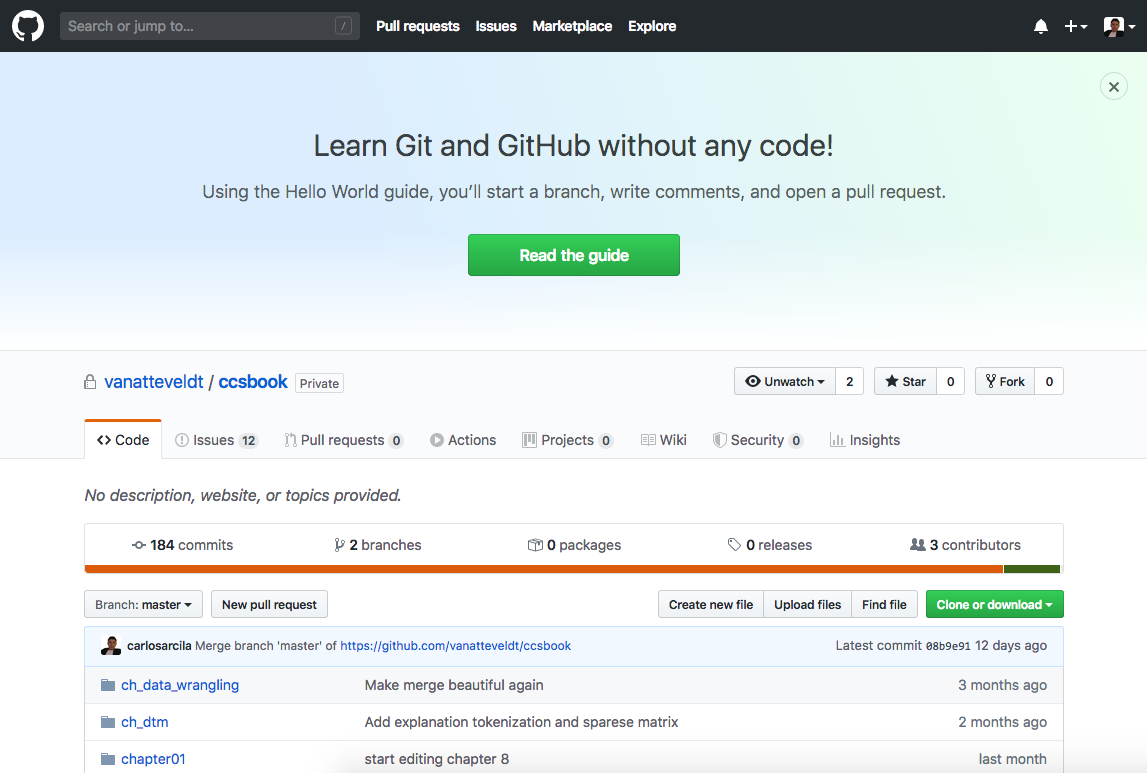
\includegraphics[width=0.9\linewidth]{figures/ch04_github}
\caption{The online repository GitHub}
\label{fig:github}
\end{figure}
 
Once you upload (or \textit{commit}) your code to GitHub you can have access to it from anywhere and will be able to track the historical changes, which in practice will allow you to have multiple versions in the very same place. You will decide if you keep the code public or private, and who to invite to edit the repository. When working collaboratively you will feel like editing a \textit{wiki} of code, while having a \textit{webpage} for your project and a \textit{net of friends} (followers), similarly to a social media. You can work locally or even from a web interface, and then synchronize the changes. When you allow colleagues to download (or \textit{clone}) your repository you are then making a good contribution to the community of developers and you can also monitor your impact. In addition to code, you can also upload other kind of files, including notebooks, and organize them in folders, just as you have it on your computer.

One extended good practice when sharing code is the use of \textit{literate programming}, which is an elegant, practical and pedagogic way to document and execute the base code. We have already mentioned in this section the importance of including documentation within your code (i.e. using the \texttt{\#} sign), but you also have the opportunity to extend this documentation (with formatted texts, images and even equations!) and put everything together to present in a logical structure all the necessary to understand the code and to run the executable lines step by step. 

There are different approaches to implement this literate programming in web and local environments, but the standard in R and Python is the use of \textit{notebooks}. In a notebook you can alternate a text processor with a executable cell to include formatted contents and blocks of code, respectively. By doing this you can include complete documentation of your scripts, and even more important you can execute each cell one step at a time (loading the results in RAM memory while the notebook is open). This last point allows you to avoid the risks of executing the whole script at once, and also to have more control of the intermediate outputs produced in your code. Once you get used to notebooks, you will probably won't want to code in a basic editor again!

The usual tool in R is the \textit{R Markdown Notebooks} and in Python the Jupyter Notebooks (see figure~\ref{fig:notebooks}), but in practice you can also deploy Python in Markdown and R in Jupyter. Both tools can help you with similar task to organize your script, though their internal technical procedures are quite different. We have chosen Jupyter to develop the examples of this book because it is a web-based interactive tool. Moreover, there several services such as Google Colab\footnote{https://colab.research.google.com}(figure~\ref{fig:colab}), that allows you remotely run these notebooks online without installing anything in your computer, making the code highly reproducible.

\begin{figure}
\centering
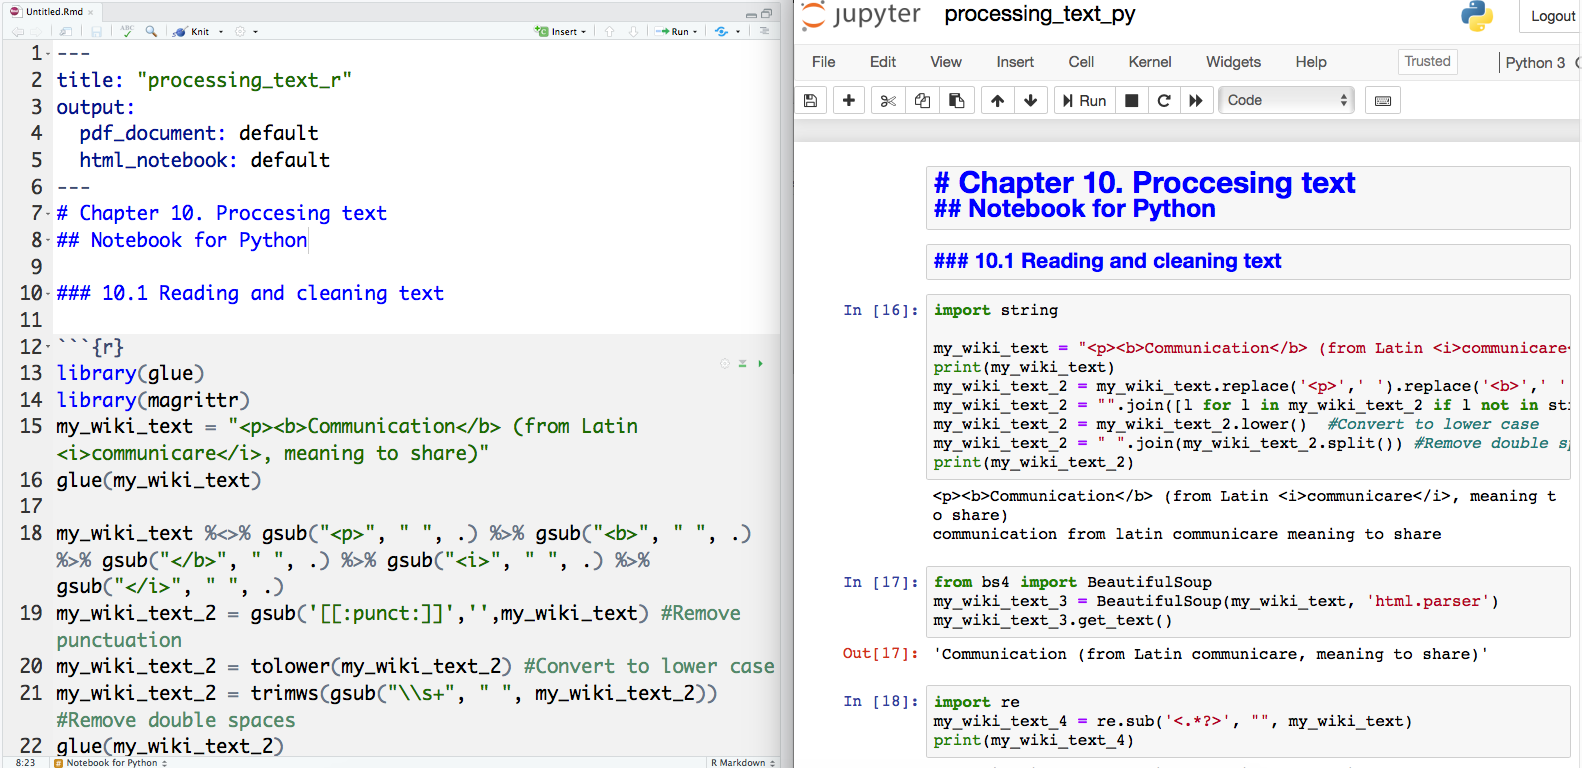
\includegraphics[width=0.9\linewidth]{figures/ch04_notebooks}
\caption{Markdown (left) and Jupyter (right) Notebooks}
\label{fig:notebooks}
\end{figure}

So far you have seen many of the possibilities that the world of code offers you from a technical and collaboration perspective. However, the practice of writing and re-using the code may also be sensitive and could lead to bad practices. The next section will deal with this ethical and normative factors.

\begin{figure}
\centering
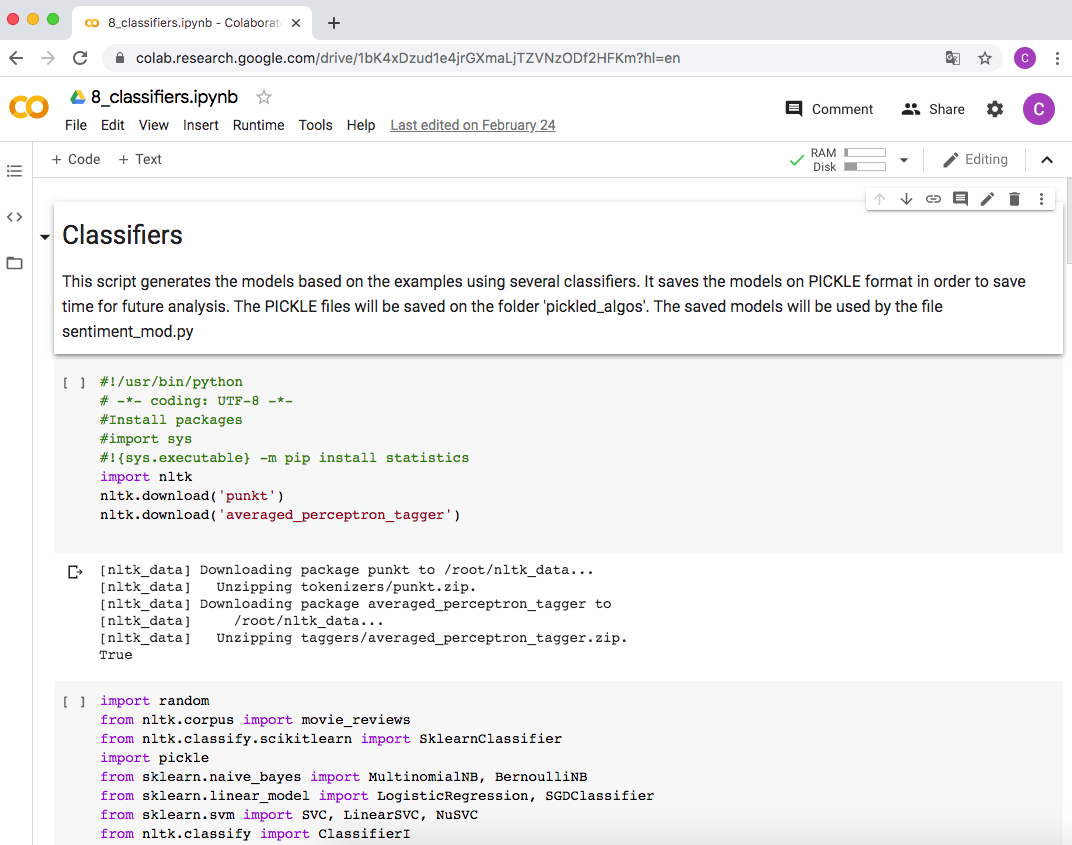
\includegraphics[width=0.9\linewidth]{figures/ch04_colab}
\caption{Jupyter notebook in Google Colab}
\label{fig:colab}
\end{figure}

